\documentclass[a4paper,11pt,notitlepage]{article}
\usepackage[utf8]{inputenc}	% latin2 - kodowanie iso-8859-2; cp1250 - kodowanie windows
\usepackage[T1]{fontenc}
\usepackage[polish]{babel}
\usepackage[MeX]{polski}
\usepackage[pdftex]{graphicx}
\selectlanguage{polish}

\usepackage{graphicx}

\hyphenation{FreeBSD}

\author{Rafał Rutyna \\ Piotr Pyśk \\ GR3}
\title{Laboratorium Sieci Komputerowych \\ {\small Interfejsy sieciowe}}
\date{\today}

\linespread{1.3}

\usepackage{indentfirst}

\begin{document}
\maketitle
\newpage
\tableofcontents
\newpage

\section{Wstęp}

\section{Program Wi-Fi Analyzer}

Za pomocą programu Wi-Fi Analyzer przeskanowaliśmy eter w budynku Starej 
Kotłowni w poszukiwaniu sieci ZETiIS i pwwifi-students.
Wyniki przedstawia rysunek~\ref{wifi-analyzer}.

\begin{figure}[htb]
  \centering
  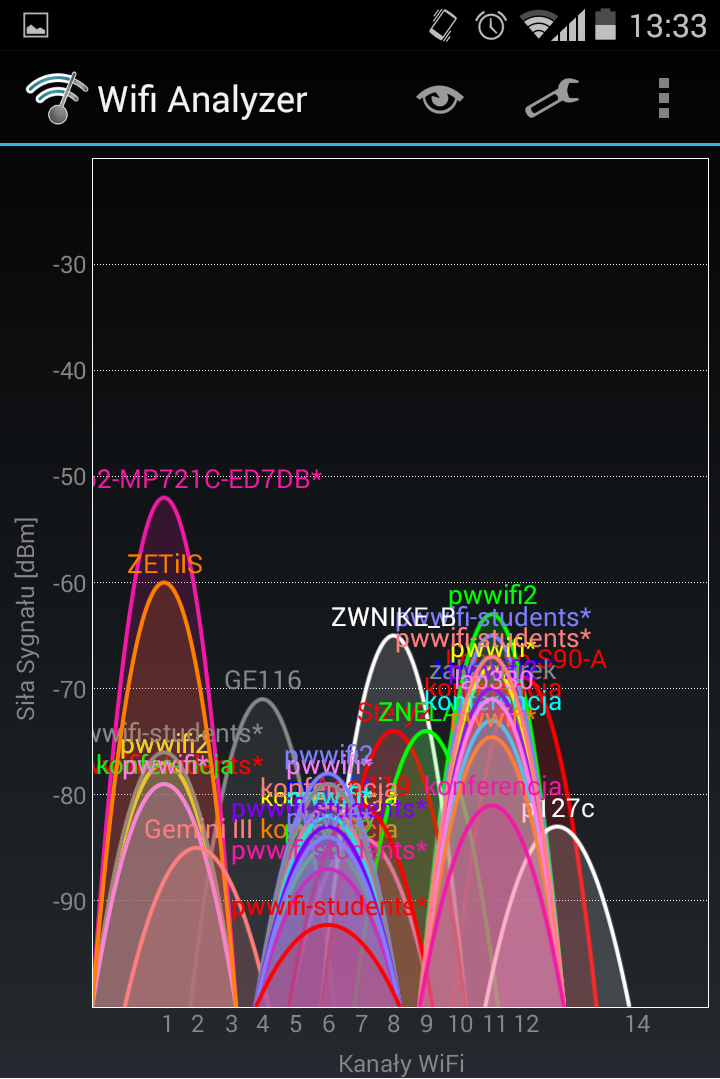
\includegraphics[width=0.5\textwidth]{analyzer.png}
  \caption{Wyniki programu Wifi-Analyzer}
  \label{wifi-analyzer}
\end{figure}


\section{Podłącznie interfejsów bezprzewodowych}

\subsection{Kreacja interfejsu wlan0}

\subsection{Połącznie z siecią pwwifi-students}

\subsection{Połącznie z siecią ZETiIS}

\section{Połącznie równy z równym}

\section{Sieć bluetooth} 

\end{document}
